\documentclass[12pt, a4paper, oneside]{book}

%===============================================
%=================FONT CHỮ======================
%===============================================
\usepackage{fontspec}
\setmainfont{DejaVu Serif}

%===============================================
%=================TOÁN HỌC======================
%===============================================
\usepackage{amsmath}
\usepackage{amssymb}
\usepackage{mathtools}
\usepackage{tikz}

%===============================================
%=================HÌNH ẢNH======================
%===============================================
\usepackage{graphicx}

%===============================================
%=================TRÌNH BÀY=====================
%===============================================
\usepackage{geometry}
\usepackage{xcolor}
\usepackage{tcolorbox}
\usepackage{indentfirst}
\usepackage{pgfplots}
\pgfplotsset{compat = 1.18}
\setlength{\parindent}{1cm}

%===============================================
%===================ĐƠN VỊ =====================
%===============================================
\usepackage{siunitx}

%===============================================
%==============LIÊN KẾT VÀ MỤC LỤC==============
%===============================================
\usepackage[plainpages=false, pdfpagelabels, hypertexnames=false]{hyperref}

\geometry{
    left = 2.5cm,
    right = 2cm,
    top = 2cm,
    bottom = 2cm
}

\title{Sổ tay công thức}
\author{Nguyễn Đức Luân}
\date{\today}

\begin{document}
    \maketitle

    \tableofcontents

    \chapter{Hàm số lượng giác và phương trình lượng giác}

\section{Giá trị lượng giác của góc lượng giác}

\subsection{Đơn vị đo góc và độ dài cung tròn}

\noindent\textbf{- Quan hệ giữa độ và radian}

\begin{center}
    $1^\circ=\dfrac{\pi}{180}\, \mathrm{rad}$ và $1\, \mathrm{rad}=\left(\dfrac{180}{\pi}\right)^\circ$
\end{center}

\noindent\textbf{- Độ dài của một cung tròn}

Một cung của đường tròn bán kính $R$ có số đo $\alpha$ rad thì có độ dài là:
\[
\fbox{$l=R.\alpha$}
\]

\subsection{Giá trị lượng giác của một góc lượng giác}

\begin{minipage}[c]{0.6\textwidth}
    \raggedright
    Xét hệ trục tọa độ Descart Oxy, ta có:\\
    + Điểm A(1;0)\\
    + Điểm A'(-1;0)\\
    + Điểm B(0,1)\\
    + Điểm B'(0,-1)\\
    \vspace{5mm}
    Giả sử điểm M(x;y) là điểm trên đường tròn lượng giác, biểu diễn góc lượng giác có số đo $\alpha$\\
    + Hoành độ $x$ của điểm M gọi là cosin của $\alpha$ và kí hiệu là $\cos\alpha$
    \[
    \cos\alpha=x
    \]
    + Tung độ $y$ của điểm M gọi là sin của $\alpha$ và kí hiệu là $\sin\alpha$
    \[
    \sin\alpha=y
    \] 
    
\end{minipage}
\hfil
\begin{minipage}[c]{0.4\textwidth}
    \centering

    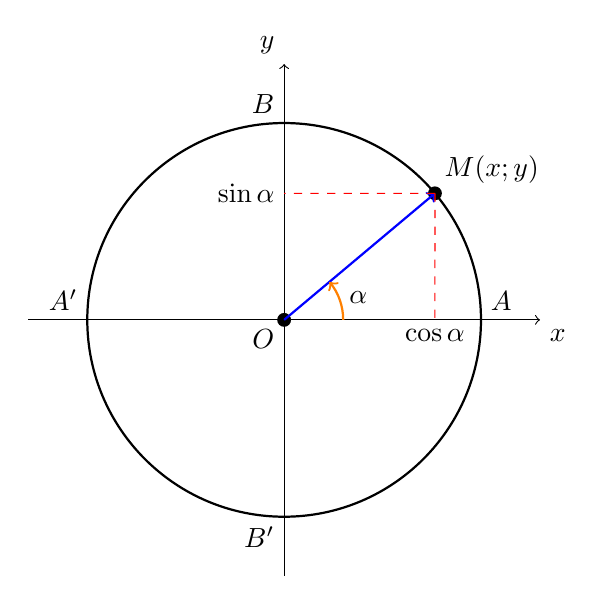
\begin{tikzpicture}[scale = 2.5]
    \def\ang{40}

    \draw[->] (-1.3, 0) -- (1.3, 0) node[below right] {$x$};
    \draw[->] (0, -1.3) -- (0, 1.3) node[above left] {$y$};

    \draw[thick] (0,0) circle(1); 

    \fill (0, 0) circle(1pt);
    \node[below left] at (0, 0) {$O$};

    \node[above right] at (1, 0) {$A$};
    \node[above left] at (0, 1) {$B$};
    \node[above left] at (-1, 0) {$A'$};
    \node[below left] at (0, -1) {$B'$};

    \coordinate (M) at ({cos(\ang)}, {sin(\ang)});

    \fill (M) circle(1pt);
    \draw[blue, thick, ->] (0, 0) -- (M);
    \node[above right] at (M) {$M(x; y)$};

    \draw[red, dashed] (M) -- (0, {sin(\ang)});
    \node[left] at (0, {sin(\ang)}) {$\sin\alpha$};

    \draw[red, dashed] (M) -- ({cos(\ang)}, 0);
    \node[below] at ({cos(\ang)}, 0) {$\cos\alpha$};

    \draw[orange, thick, ->] (0.3, 0) arc (0:\ang:0.3);
    \node[above right] at ({0.3 * cos(\ang / 2)}, {0.1 * sin(\ang / 2)}) {$\alpha$};

\end{tikzpicture}
\end{minipage}

+ Nếu $\cos\alpha\neq0$, tỉ số $\dfrac{\sin\alpha}{\cos\alpha}$ gọi là tang của $\alpha$ và kí hiệu là $\tan\alpha$:
\[
\fbox{$\tan\alpha=\dfrac{\sin\alpha}{\cos\alpha}$}
\]

+ Nếu $\sin\alpha\neq0$, tỉ số $\dfrac{\cos\alpha}{\sin\alpha}$ gọi là costang của $\alpha$ và kí hiệu là $\cot\alpha$:
\[
\fbox{$\cot\alpha=\dfrac{\cos\alpha}{\sin\alpha}$}
\]

\noindent\textbf{Chú ý:} Ta cũng gọi trục tung là trục \textbf{sin}, còn trục hoành là trục \textbf{cos}

\subsection{Quan hệ giữa các giá trị lượng giác}

\noindent\textbf{- Công thức lượng giác cơ bản}\\

\par
+ Đối với các giá trị lượng giác, ta có các hằng đẳng thức sau\\
\[
    \begin{aligned}
        &\fbox{$\sin^2\alpha+\cos^2\alpha=1$}\\[6pt]
        &\fbox{$1+\tan^2\alpha=\dfrac{1}{\cos^2\alpha}$},\quad \alpha\neq\dfrac{\pi}{2}+k\pi,\quad k\in\mathbb{Z}\\[6pt]
        &\fbox{$1+\cot^2\alpha=\dfrac{1}{\sin^2\alpha}$},\quad \alpha\neq k\pi,\quad k\in\mathbb{Z}\\[6pt]
        &\fbox{$\tan\alpha.\cot\alpha=1$}, \quad \alpha \neq \dfrac{k\pi}{2}, \quad k \in \mathbb{Z}
    \end{aligned}
\]

\noindent\textbf{- Giá trị lượng giác của các góc có liên quan đặc biệt}
\par
+ Góc đối nhau:
\[
    \begin{aligned}
        &\fbox{$\cos(-\alpha)=\cos\alpha$}\\[6pt]
        &\fbox{$\sin(-\alpha)=-\sin\alpha$}\\[6pt]
        &\fbox{$\tan(-\alpha)=-\tan\alpha$}\\[6pt]
        &\fbox{$\cot(-\alpha)=-\cot\alpha$}\\[6pt]
    \end{aligned}
\]

+ Góc bù nhau:
\[
    \begin{aligned}
        &\fbox{$\cos(\pi-\alpha)=-\cos\alpha$}\\[6pt]
        &\fbox{$\sin(\pi-\alpha)=\sin\alpha$}\\[6pt]
        &\fbox{$\tan(\pi-\alpha)=-\tan\alpha$}\\[6pt]
        &\fbox{$\cot(\pi-\alpha)=-\cot\alpha$}\\[6pt]
    \end{aligned}
\]

+ Góc phụ nhau:
\[
    \begin{aligned}
        &\fbox{$\cos\left(\dfrac{\pi}{2}-\alpha\right)=\sin\alpha$}\\[6pt]
        &\fbox{$\sin\left(\dfrac{\pi}{2}-\alpha\right)=\cos\alpha$}\\[6pt]
        &\fbox{$\tan\left(\dfrac{\pi}{2}-\alpha\right)=\cot\alpha$}\\[6pt]
        &\fbox{$\cot\left(\dfrac{\pi}{2}-\alpha\right)=\tan\alpha$}\\[6pt]
    \end{aligned}
\]

+ Góc hơn kém $\pi$:
\[
    \begin{aligned}
        &\fbox{$\cos(\pi+\alpha)=-\cos\alpha$}\\[6pt]
        &\fbox{$\sin(\pi+\alpha)=-\sin\alpha$}\\[6pt]
        &\fbox{$\tan(\pi+\alpha)=\tan\alpha$}\\[6pt]
        &\fbox{$\cot(\pi+\alpha)=\cot\alpha$}\\[6pt]
    \end{aligned}
\]

+ Góc hơn kém $\dfrac{\pi}{2}$:
\[
    \begin{aligned}
        &\fbox{$\cos\left(\dfrac{\pi}{2}+\alpha\right)=-\sin\alpha$}\\[6pt]
        &\fbox{$\sin\left(\dfrac{\pi}{2}+\alpha\right)=\cos\alpha$}\\[6pt]
        &\fbox{$\tan\left(\dfrac{\pi}{2}+\alpha\right)=-\cot\alpha$}\\[6pt]
        &\fbox{$\cot\left(\dfrac{\pi}{2}+\alpha\right)=-\tan\alpha$}\\[6pt]
    \end{aligned}
\]

\section{Công thức lượng giác}

\subsection{Công thức cộng}
\[
    \begin{aligned}
        &\fbox{$\cos(\alpha\pm\beta)=\cos\alpha\cos\beta\mp\sin\alpha\sin\beta$}\\[6pt]
        &\fbox{$\cos(\alpha\pm\beta)=\cos\alpha\cos\beta\pm\sin\alpha\sin\beta$}\\[6pt]
        &\fbox{$\tan(\alpha\pm\beta)=\dfrac{\tan\alpha\pm\tan\beta}{1\mp\tan\alpha\tan\beta}$}
    \end{aligned}
\]

\subsection{Công thức hạ bậc}
\[
    \begin{aligned}
        &\fbox{$\cos^2\alpha=\dfrac{1+\cos2\alpha}{2}$}\\[6pt]
        &\fbox{$\sin^2\alpha=\dfrac{1-\cos2\alpha}{2}$}\\[6pt]
        &\fbox{$\tan^2\alpha=\dfrac{1-\cos2\alpha}{1+\cos2\alpha}$}
    \end{aligned}
\]

\subsection{Công thức biến đổi tính thành tổng}
\[
    \begin{aligned}
        &\fbox{$\cos\alpha\cos\beta=\dfrac{1}{2}[\cos(\alpha-\beta)+\cos(\alpha+\beta)]$}\\[6pt]
        &\fbox{$\sin\alpha\sin\beta=\dfrac{1}{2}[\cos(\alpha-\beta)-\cos(\alpha+\beta)]$}\\[6pt]
        &\fbox{$\sin\alpha\cos\beta=\dfrac{1}{2}[\sin(\alpha-\beta)+\sin(\alpha+\beta)]$}
    \end{aligned}
\]

\subsection{Công thức biến đổi tổng thành tích}
\[
    \begin{aligned}
        &\fbox{$\cos\alpha+\cos\beta=2\cos\left(\dfrac{\alpha+\beta}{2}\right)\cos\left(\dfrac{\alpha-\beta}{2}\right)$}\\[6pt]
        &\fbox{$\cos\alpha-\cos\beta=-2\sin\left(\dfrac{\alpha+\beta}{2}\right)\sin\left(\dfrac{\alpha-\beta}{2}\right)$}\\[6pt]
        &\fbox{$\sin\alpha+\sin\beta=2\sin\left(\dfrac{\alpha+\beta}{2}\right)\cos\left(\dfrac{\alpha-\beta}{2}\right)$}\\[6pt]
        &\fbox{$\sin\alpha-\sin\beta=2\cos\left(\dfrac{\alpha+\beta}{2}\right)\sin\left(\dfrac{\alpha-\beta}{2}\right)$}
    \end{aligned}
\]

\section{Hàm số lượng giác}

\subsection{Hàm số chẵn, hàm số lẻ}

- Cho hàm số lượng giác $y=f(x)$ có tập xác định là $D$.\\[6pt]
\hspace*{1.3cm}
+ Hàm số $f(x)$ được gọi là \textcolor{red}{hàm số chẵn} nếu
\[
    \begin{cases}
        \forall x \in D \rightarrow -x \in D \\
        f(-x) = f(x)
    \end{cases}
\]
\hspace*{1.3cm}
+ Hàm số $f(x)$ được gọi là \textcolor{red}{hàm số lẻ} nếu
\[
    \begin{cases}
        \forall x \in D \rightarrow -x \in D\\
        f(-x) = -f(x)
    \end{cases}
\]

\noindent\textbf{Chú ý:}\\
\hspace*{1cm}
+ Đồ thị của một \textcolor{red}{hàm số chẵn} nhận trục tung là trục đối xứng\\
\hspace*{1cm}
+ Đồ thị của một \textcolor{red}{hàm số lẻ} nhận gốc tọa độ là tâm đối xứng

\subsection{Hàm số tuần hoàn}
- Hàm số $y=f(x)$ có tập xác định $D$ được gọi là \textcolor{red}{hàm số tuần hoàn} nếu tồn tại số $T \neq 0$ sao cho với mọi $x \in D$, ta có:
\[
    \begin{cases}
        x \pm T \in D\\
        f(x \pm T) = f(x)
    \end{cases}
\]

- Số $T > 0$ nhỏ nhất thỏa mã các điều kiện trên (nếu có) được gọi là \textcolor{red}{chu kì} của hàm số tuần hoàn đó.

\subsection{Đồ thị và tính chất của hàm số $y=\sin x$}
\noindent
\hspace*{1cm}
- Tập xác định: $D = \mathbb{R}$\\[6pt]
\hspace*{1cm}
- Tập giá trị: $[-1;1]$\\[6pt]
\hspace*{1cm}
- Là hàm số lẻ vì: $\sin(-x) = -\sin x, \quad \forall x \in \mathbb{R}$\\[6pt]
\hspace*{1cm}
- Là hàm số tuần hoàn với chu kỳ: $T = 2 \pi$\\[6pt]
\hspace*{1cm}
- Hàm số $y = \sin x$ nhận các giá trị đặc biệt:\\[6pt]
\[
    \begin{aligned}
        &\fbox{$\sin x = 0 \iff x = k \pi, \quad k \in \mathbb{Z}$}\\[6pt]
        &\fbox{$\sin x = 1 \iff x = \dfrac{\pi}{2} + k2\pi, \quad k \in \mathbb{Z}$}\\[6pt]
        &\fbox{$\sin x = -1 \iff x = -\dfrac{\pi}{2} + k2\pi, \quad k \in \mathbb{Z}$}
    \end{aligned}
\]
\hspace*{1cm}
- Đồ thị hàm số $y = \sin x$:\\
\begin{center}
    \centering
    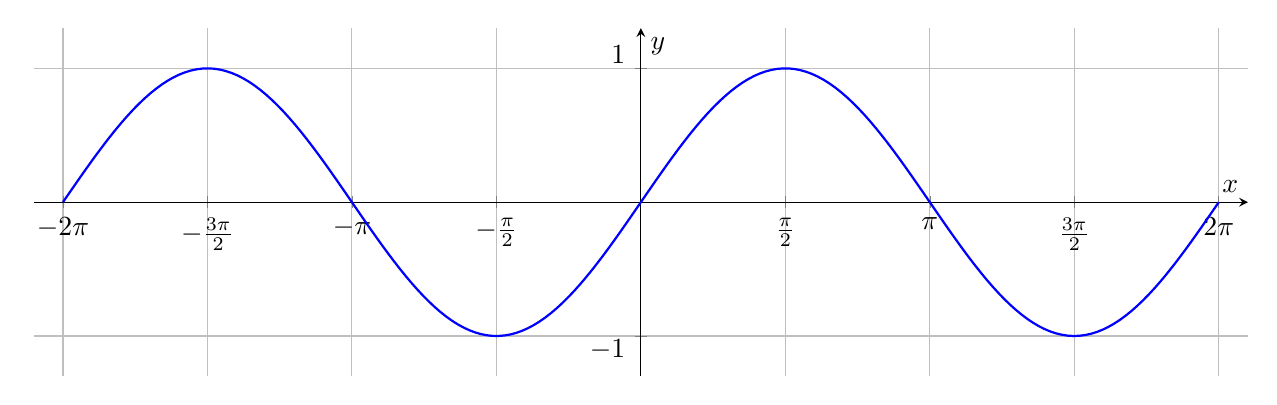
\begin{tikzpicture}
    \begin{axis}
        [
            width = 17cm,
            height = 6cm,
            axis lines = middle,
            xlabel = {$x$},
            ylabel = {$y$},
            xmin = -6.6,
            xmax = 6.6,
            ymin = -1.3,
            ymax = 1.3,
            xtick = {-6.2832, -4.7124, -3.1415, -1.5708, 0, 1.5708, 3.1415, 4.7124, 6.2832},
            xticklabels={
                    $-2\pi$,
                    $-\frac{3\pi}{2}$,
                    $-\pi$,
                    $-\frac{\pi}{2}$,
                    $0$,
                    $\frac{\pi}{2}$,
                    $\pi$,
                    $\frac{3\pi}{2}$,
                    $2\pi$
                },            
            ytick = {-1, 0, 1},
            yticklabel style = {yshift = {\tick*5pt}},
            grid = major, 
        ]

        \addplot
        [
            blue,
            thick,
            domain = -6.2832:6.2832,
            samples = 200
        ] {sin(deg(x))};
    \end{axis}
\end{tikzpicture}

\end{center}

\subsection{Đồ thị và tính chất của hàm số $y = \cos x$}
\noindent
\hspace*{1cm}
- Tập xác định: $D = \mathbb{R}$\\[6pt]
\hspace*{1cm}
- Tập giá trị: $[-1;1]$\\[6pt]
\hspace*{1cm}
- Là hàm số chẵn vì: $\cos(-x) = \cos x, \quad \forall x \in \mathbb{R}$\\[6pt]
\hspace*{1cm}
- Là hàm số tuần hoàn với chu kỳ: $T = 2 \pi$\\[6pt]
\hspace*{1cm}
- Hàm số $y = \cos x$ nhận các giá trị đặc biệt:\\[6pt]
\[
    \begin{aligned}
        &\fbox{$\cos x = 0 \iff x = \dfrac{\pi}{2} + k\pi, \quad k \in \mathbb{Z}$}\\[6pt]
        &\fbox{$\cos x = 1 \iff x = k2\, \quad k \in \mathbb{Z}$}\\[6pt]
        &\fbox{$\cos x = -1 \iff x = \pi + k2\pi, \quad k \in \mathbb{Z}$}
    \end{aligned}
\]
\hspace*{1cm}
- Đồ thị hàm số $y = \cos x$:\\
\begin{center}
    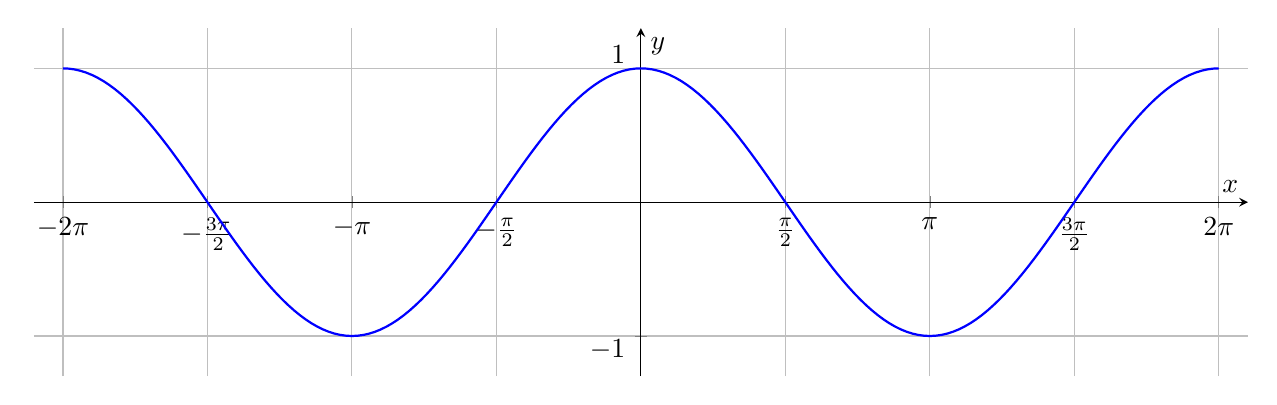
\begin{tikzpicture}
    \begin{axis}
        [
            width = 17cm,
            height = 6cm,
            axis lines = middle,
            xlabel = {$x$},
            ylabel = {$y$},
            xmin = -6.6,
            xmax = 6.6,
            ymin = -1.3,
            ymax = 1.3,
            xtick = {-2*pi, -3*pi/2, -pi, -pi/2, 0, pi/2, pi, 3*pi/2, 2*pi},
            xticklabels = {
                    $-2\pi$,
                    $-\frac{3\pi}{2}$,
                    $-\pi$,
                    $-\frac{\pi}{2}$,
                    $0$,
                    $\frac{\pi}{2}$,
                    $\pi$,
                    $\frac{3\pi}{2}$,
                    $2\pi$
                },
            ytick = {-1, 0, 1},
            yticklabel style = {yshift = {\tick*5pt}},
            grid = major,
        ]

        \addplot
        [
            blue,
            thick,
            domain = -2*pi:2*pi,
            samples = 201
        ] {cos(deg(x))};
    \end{axis}
\end{tikzpicture}

\end{center}

\subsection{Đồ thị và tính chất của hàm số $y = \tan x$}

\end{document}